\documentclass[10pt, oneside]{article} 
\usepackage{amsmath, amsthm, amssymb, calrsfs, wasysym, verbatim, bbm, color, graphics, geometry, gensymb}

\usepackage{graphicx}

\geometry{tmargin=.75in, bmargin=.75in, lmargin=.75in, rmargin = .75in}  

\newcommand{\R}{\mathbb{R}}
\newcommand{\C}{\mathbb{C}}
\newcommand{\Z}{\mathbb{Z}}
\newcommand{\N}{\mathbb{N}}
\newcommand{\Q}{\mathbb{Q}}
\newcommand{\norm}[1]{\left\lVert#1\right\rVert}
\newcommand{\Cdot}{\boldsymbol{\cdot}}

\newtheorem{thm}{Theorem}
\newtheorem{defn}{Definition}
\newtheorem{conv}{Convention}
\newtheorem{rem}{Remark}
\newtheorem{lem}{Lemma}
\newtheorem{cor}{Corollary}

\usepackage[hidelinks]{hyperref}

\title{CS 334}
\author{Alexander Liu}
\date{Fall 2024}

\begin{document}

\maketitle
\tableofcontents

\vspace{.25in}

\section{Intro}
\subsection{Basics}
\begin{itemize}
    \item What is machine learning?
    \begin{itemize}
        \item In classical programming, we give the rules + data to get answers
        \item In ML, we put in data and answers to get the rules
        \item Many types \& applications: supervised learning (follow correct behavior), unsupervised learning (look for patterns in data), reinforcement learning (figure out how to achieve good outcomes)
        \begin{itemize}
            \item Mainly focus on supervised learning
            \item A bit of unsupervised learning
            \begin{itemize}
                \item Clustering, collaborative filtering
            \end{itemize}
            \item A bit of Reinforcement Learning
        \end{itemize}
    \end{itemize}
    \item We use NumPy, Pandas, Matplotlib, Pytorch, Scikit Learn
\end{itemize}

\subsection{Binary Classification}
\begin{itemize}
    \item Two possible outcomes
    \begin{itemize}
        \item Is this email a spam?
        \item Is this review positive?
        \item Is this digit a ``9"?
        \item Is this image a Chihuahua or a muffin?
    \end{itemize}
    \item Feature vector: $\{\vec{x}^{(1)}, y^{(1)}\}$, where $\vec{x}$ is a d-dimensional feature vector, and $y$ is a label
    \begin{itemize}
        \item Here, since we are using a binary classifier, our ``label space" is $\{-1,+1\}$
    \end{itemize}
    \item Given training data containing a set of labeled examples, come up with a rule that maps an unable example to the correct label
    \item \textbf{Objective:} Given $\{\vec{x}^{(1)}, y^{(1)}\}$, where $\vec{x}^N _{i=1}$ where $\vec{x}^{(1)}\in \R^d, y^{(i)}\in {-1,+1}$, find a ``good`` $h:\R^d \rightarrow \{-1,+1\}$

\end{itemize}

Make sure to label plots.
We can and should look up documentation online
Can use seaborn, matplotlib, pandas, numpy

\subsection{Linear Classification}
\begin{itemize}
    \item feature vector $\vec{x} = [x_1,x_2,...,x_d]^T$ (transpose to indicate column vector), $\vec{x} \in \R^d$
    \item label $y\in \{-1,+1\}$
    \item training set of labeled training $D=\{\vec{x}^{(i)}, y^{(i)}\}^N _{i=1}$. In English, paired/zipped up feature vectors and labels
    \item classifier: $h:\R^d \rightarrow \{-1, +1\}$. $h(\vec{x}) = h(x_1, x_2,...,x_d)$
    \item Goal: select the best $h$ from a set of possible classifiers $\mathbb{H}$ that would have the best change of classifying new examples
    \item Example
    \begin{itemize}
        \item Let $\vec{x} = [x_1, x_2, ..., x_{360}]^T, x_k \in \{1,...,2048\}$
        \item Suppose a training set of $N=100, D= {\vec{x} ^(i) , y^{(i)}}\} ^{100} _ {i=1}$ where $x_3$ is different in every example.
        \item Build a lookup table.
        $h(\vec{x}) =$
        \begin{itemize}
            \item $y^{(i)}$ if $x_3 = x_3 ^{(i)}$
            \item $-1$ otherwise
        \end{itemize}
        \item Is this a good classifier? NO. We just default to $-1$ if we don't have a match
        \item We want Generalization. In other words, works well on unseen examples.
        \item In this case, the classifier overfits (to the training data)
        \item Problem: too many choices in $\mathbb{H}$. We need to constrain what $\mathbb{H}$ can be.
        \item Solution here: constrain $\mathbb{H}$ to a linear classifier. However, this can't be too small (ex: if we only have 1 possible value, then we will just be inaccurate)
        \item Important to find the right balance $\rightarrow$ model selection

    \end{itemize}
    \item Linear Classifiers (through the origin)
    \begin{itemize}
        \item Thresholded linear mapping from feature vectors to labels.
        \item $h(\vec{x}; \vec{\theta}) = \{-1 \text{ if } \vec{\theta} \cdot \vec{x} \geq 1, +1 \textbf{ if } \vec{\theta}\cdot \vec{x} < 1\},\text{   } \vec{\theta} = [\theta_1,\theta_2, ..., \theta_d]^T$, where semicolon indicates input vs output
        \item $\vec{\theta} \cdot \vec{x}$ is element-wise dot product
        \item Different $\vec{\theta}$'s produce potentially different labeling for the same $\vec{x}$
        \item $\vec{\theta}$ defines a hyperplane that goes through the origin, dividing the feature space into a positive side and a negative side
        \begin{itemize}
            \item We call the hyperplane ($\theta_2)$?) the ``decision boundary". It is orthogonal to the label vector $\theta$
            \item What happens if a point is on the hyperplane?
            \begin{itemize}
                \item $\vec{\theta} \cdot \vec{x} = \norm{\vec{\theta}}\norm{\vec{x}}cos90\degree = 0$
                \item $x_2 = - \frac{\theta_1}{\theta_2}x_1$, where $-\frac{\theta_1}{\theta_2}$ is the slope
                \item Does length matter? No.
                \item Does direction matter? Yes because it affects the angle
            \end{itemize}
        \end{itemize}
    \end{itemize}
    \item How do we select $\vec{\theta}$?
    \begin{itemize}
        \item Intuition: find a $\vec{\theta}$ that works well on the training data.
        \item Why is this ok now? Didn't we say overfit?
        \item Now we've constrained $\mathbb{H}$ to linear, reducing the change of overfitting
        \item Minimize Training Error
        \begin{itemize}
            \item Training Error: fraction of training examples for which the classifier predicts the wrong labels
        \end{itemize}
        \item $\varepsilon_N (\vec{\theta}) = \frac{1}{N} \sum_{i=1} ^N \mathbb{I} [y^{(i)} \neq h(\vec{x} ^{(i)} ; \vec{\theta})]$ \\$= \frac{1}{N} \sum_{i=1} ^N \mathbb{I}[y^{(i)} (\vec{\theta} \cdot \vec{x} ^{(i)}) \leq 0]$, where $\mathbb{I}[\cdot]$ returns $1$ if logical equation evaluates to true, $0$ otherwise
    \end{itemize}
\end{itemize}

\subsection{Dot Product}
\begin{itemize}
    \item $\vec{\theta} \cdot \vec{x} = \norm{\vec{\theta}}\norm{\vec{x}} cos\alpha$, where $\alpha$ is the angle between the two vectors
    \item Recall norm: $\norm{\vec{x}} = \sqrt{x_1^2 + x_2 ^2 + ... + x_d^2} \geq 0$
\end{itemize}

\subsection{Linear Classifier through the origin}
\begin{itemize}
    \item $h(\vec x; \vec \theta) = sign(\vec \theta \cdot \vec x)= $+1 if dot product > 0, 0 if dot product = 0, -1 if theta < 0.
    \begin{itemize}
        \item In binary case, we have to make 0 as +1 or -1
    \end{itemize}
    \item $\vec \theta$ faces positive side, where $\vec \theta \cdot \vec x = 0$ defines a hyperplane: decision boundary
    \item Training Error: $\epsilon_N (\vec \theta) = \frac{1}{N}\sum_{i=1} ^N I[]$complete later
\end{itemize}

\subsection{Linear Classifier with offset}
\begin{itemize}
    \item $h(\vec x; \vec \theta, b) =sign(\vec \theta \cdot \vec x + b), \vec x \in \R^d, \vec \theta \in \R^d, b\in \R$
    \item New decision boundary $\vec \theta \cdot \vec x + b= 0$ doesn't pass through the origin (when $b\neq 0$).
    \item $\vec \theta \cdot \vec x + b = 0$ is ``parallel" to $\vec \theta \cdot \vec x+b=\vec \theta \cdot \vec x$ which is only possible when b=0
    \item Signed distance between two decision boundaries: $\frac{-b}{||\vec\theta||}$ from $\vec \theta\cdot \vec x=0$. Why?
    \begin{itemize}
        \item Point from decision boundary 1: $\vec \theta \cdot \vec x^{(1)} 0$
        \item Point from offset decision boundary 2: vector from $\vec x ^{(1)}$ to $\vec x^{(2)} \vec v = \vec x ^{(2)} - \vec x^{(1)}$ orthogonal projection
        \item $proj_{\vec \theta} \vec v= (\frac{\vec v \cdot \vec \theta}{||\vec \theta||}) \frac{\vec \theta}{||\vec \theta||}$. Second part is unit vector, so we just want the first part (scalar)
        \[
        = \frac{\vec{v} \cdot \vec{\theta}}{||\vec{\theta}||}
        = \frac{\left( \vec{x}^{(2)} - \vec{x}^{(1)} \right) \cdot \vec{\theta}}{||\vec{\theta}||}
        = \frac{\vec{x}^{(2)} \cdot \vec{\theta} - \vec{x}^{(1)} \cdot \vec{\theta}}{||\vec{\theta}||}
        = \frac{-b}{||\vec{\theta}||}
        \]
        \item b is negative above because for offset: $\vec \theta \cdot \vec x = -b$
        \item Definition: $D=\{\vec x ^{(i)}, y^{(i)}\}_{i=1}^N$ are linearly separable through the irign if there exists$\vec \theta$ such that $y^{(i)} (\vec \theta \cdot \vec x^{(i)}) > 0, \forall i= 1\cdots N$. Basically can we find a theta that can separate all points
        \item \textbf{Perceptron Algorithm}
        \begin{itemize}
            \item Mistake-driven: starts with $\vec \theta = \vec 0$ (zero vector) and $k=0$, tries to update $\vec \theta$ to correct any mistakes. At first, all points are misclassified
            \item While not all points are not correctly classified. Loop through all points. $y$ is the label, $x$ is the feature vector
            \begin{itemize}
                \item If $y^{(i)}(\vec \theta \cdot \vec x^{(i)})\leq 0$ \textbf{(INCORRECT CLASSIFICATION)}, set $\vec \theta^{(k+1)} =\vec \theta^{(k)} + y^{(i)} \vec x^{(i)}$, $k$++
                \item Inner boolean: only update i.f.f incorrect classification
            \end{itemize}
            \item The reason why we need multiple passes is because even on update we may ``undershoot" on an update for a current point, continuing to leave it misclassified
            \item Suppose we make a mistake on $\vec x^{(i)}$ and update $y^{(i)} (\vec \theta ^{(k)} \cdot \vec x ^{(i)})\leq 0$. Suppose we still misclassify after update: $y^{(i)} (\vec \theta ^{(k+1)} \cdot \vec x^{(i)} )\leq 0$, where $\vec \theta ^{(k+1)} = \vec \theta ^{(k)} + y^{(i)}\vec x^{(i)}$. We need to iterate again
            \begin{thm} {Convergence of perception:the perception algorithm converges after a finite number of mistakes if the training examples are linearly separable (through the origin)}\end{thm}
            \item We don't really use this algorithm because if it's not linearly separable, it runs on forever. The output may not even be good (only does the minimum to make sure it fits the training data). However, it is the building block for a lot of other concepts
        \end{itemize}
    \end{itemize}
\end{itemize}

\section{Our First Linear Classifier: Perceptron}
\subsection{Perception}

Perceptron algorithm was proposed in 1958
\begin{itemize}
    \item Mark 1 Perceptron: was meant to be a machine
\end{itemize}

Perceptron with offset (add b to represent y offset)
\begin{itemize}
    \item $k=0, \vec \theta^{(0)} = \vec 0, b^{(0)} = 0$
    \item while not all points are correctly classified
    \item if $y^{(0)} (\vec \theta ^{(k)} \cdot \vec x^{(k)} + b)\leq0$
    \begin{itemize}
        \item $\vec \theta^{(k+1)} = \vec \theta^{(k)} + y^{(i)} \vec x^{(i)}$
        \item $b^{(k+1)}= b^{(k)} + y^{(i)}$
        \item $k = k+1$
    \end{itemize}
\end{itemize}
\textbf{Convergence Theorem}
\begin{itemize}
    \item If the training data set is linearly separable, the perception is guaranteed to converge (find a valid decision boundary) after a finite number of updates
    \item However
    \begin{itemize}
        \item No guarantee on uniqueness of solutions
        \item ``finite number" of updates doesn't fit a specific constraint. Can be large
        \begin{itemize}
            \item ``undershoot" when current point remains misclassified after update
            \item Previously correct data point may become misclassified after update
        \end{itemize}
    \end{itemize}
\end{itemize}
The Perceptron failed on the convergence and needs to have a \textbf{`PERFECT'
(no wrong outputs in training data)} decision boundary (linearly separable)
\begin{itemize}
    \item The ``famous XOR problem" (Minsky and Papert, “Perceptrons”, 1969.): a perfect decision boundary does not exist
    \item The perception algorithm would run indefinitely and never converge (remember it's not guaranteed to find a solution that minimizes training error)
\end{itemize}
Training Error
\begin{itemize}
    \item $\epsilon_N(\vec \theta) = \frac{1}{N} \sum_{i=1} ^n I[y^{(i)} (\vec \theta \cdot \vec x ^{(i)}) \leq 0]$
\end{itemize}
\subsection{Empirical Risk and Zero-One Loss Problems}
Empirical Risk
\begin{itemize}
    \item $R_N (\vec \theta) = \frac{1}{N} \sum_{i=1} ^N loss(y^{(i)}(\vec \theta \cdot \vec x ^{(i)}))$
    \item Divide by N to get average of sum of loss function
    \item Previously, we were looking at the ``zero-one loss"
    \begin{itemize}
        \item Let $z=y(\vec \theta \cdot \vec x)$
        \item $loss_{0-1} (z) = I(z\leq 0)= $ $ \begin{cases} 
          1 & \text{if } z \leq 0 \\
         0 & \text{otherwise} \\
        \end{cases}$
        \item Binary piecewise function
        \item \textbf{Problems (mainly continuity and horizontal line that doesn't maintain context well)}
        \begin{itemize}
            \item Not continuous at $z=0$
            \item Not differentiable at $z=0$
            \item not convex (concave-up (U, bowl-shape), no second-order derivative)
        \end{itemize}
        \item Another problem: we don't penalize mistakes based on their distance from the decision boundary. They are all treated equally: ``A mistake is a mistake"
        \begin{itemize}
            \item We can fix these problems with hinge-loss (looks like a horizontally flipped and shifted ReLU kinda)
        \end{itemize}
    \end{itemize}
\end{itemize}

\textbf{How do we approach data that is not linearly separable?}
\subsection{Necessary Conditions for Gradient Descent}
\begin{itemize}
    \item Continuous
    \item Differentiable
    \item Convex (we have at least one local/global minimum)
\end{itemize}

\subsection{Hinge Loss}
\begin{itemize}
    \item Designed to penalize misclassifications the further away they are from our decision boundary
    \item $loss_h (z) = max\{0,1-z\}$
    \begin{itemize}
        \item Now, loss increases linearly as z decreases
    \end{itemize}
    \item $z=y(\vec \theta \cdot \vec x)$
    \item $y(\vec \theta\cdot x)$
    \begin{itemize}
        \item sign: +/-
        \item magnitude
        \begin{itemize}
            \item $|y(\vec \theta\cdot \vec x)|=|y||\vec\theta\cdot \vec x|= |\pm 1| |\vec \theta\cdot \vec x| = |\vec \theta\cdot \vec x|$ is proportional to the distance $\frac{|\vec \theta \cdot \vec x|}{||\vec \theta||}$
        \end{itemize}
    \end{itemize}
    \item Since hinge loss is \textbf{continuous, differentiable, convex}, we have a simple algo. to minimize \textbf{``Gradient Descent"}
\end{itemize}
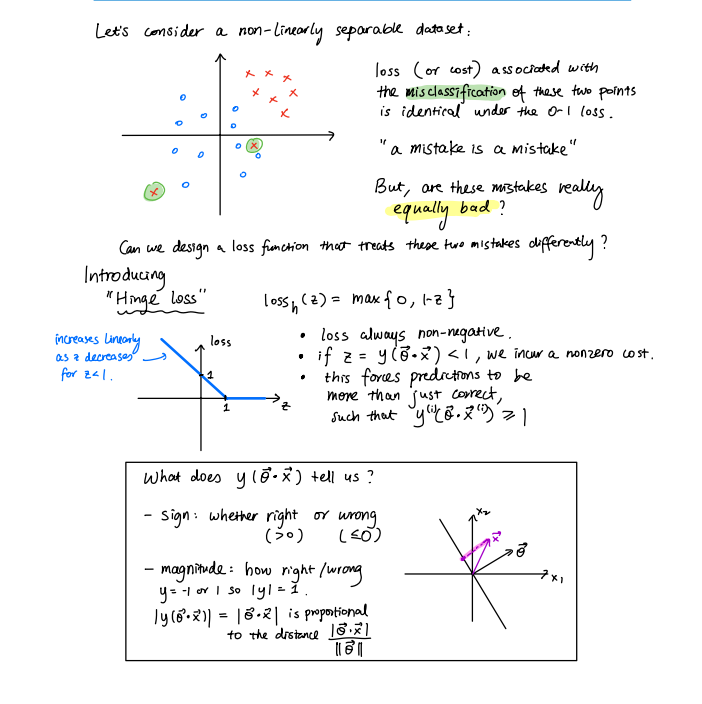
\includegraphics[scale=0.9]{Images/hinge_loss.png}

To clarify, empirical risk is NOT a loss function, it is taking the average of the output of a loss function. In other words, it is a function of the loss function

\subsection{Quick Calculus Review}
\begin{itemize}
    \item $y=f(\vec x)=f(x_1,x_2,\cdots,x_d)$
    \item Partial derivative: $\frac{\partial f}{\partial x_j} : \R^d\rightarrow \R$, ``rate of change in one axis direction"
    \item ``if differentiating with $x_j$, I'll treat the rest of x as constants"
    \item Gradient: $\nabla_{\vec x} f(\vec x) = [\frac{\partial}{\partial x_1} f(\vec x), \frac{\partial}{\partial x_2} f(\vec x),\cdots, \frac{\partial}{\partial x_d} f(\vec x)]^T$
    \begin{itemize}
        \item $\nabla_{\vec x} f(\vec x) : \R^d \rightarrow \R^d$ is a vector-valued function
        \item Gradient is a normal vector
        \item \textbf{In which direction does f increase the fastest?} The gradient vector
        \item Gradient descent
        \begin{itemize}
            \item Suppose we want to minimize $f(\vec \theta)$ with $\vec \theta$. We know gradient $\nabla_{\vec \theta} f(\vec \theta)$ points in the direction of the steepest increase.
            \begin{itemize}
                \item For gradient descent, we take small steps in opposite direction of gradient
                \item $\vec \theta^{(0)} = \vec 0, k=0$ while not converged
                \item |$\vec \theta^{(k+1)} = \vec \theta ^{(k)} - n_k \nabla_{\vec \theta} f(\vec \theta) |_{(\vec \theta = \vec \theta^{(k)})}$
            \end{itemize}
        \end{itemize}
    \end{itemize}
\end{itemize}

\subsection{Gradient Descent}
Suppose we want to minimize some $f(\vec \theta): \R^d \rightarrow \R$ (some function e.g. empirical risk) with respect to $\vec \theta$. We know gradient $\nabla_{\vec\theta}f(\vec \theta)$ points in the direction of \textbf{steepest increase}.
\begin{itemize}
    \item Idea: take a small step in the \textbf{opposite direction}
    \begin{itemize}
        \item $\vec \theta ^{(0)} = \vec \theta, k=0$
        \item While not converged
        \begin{itemize}
            \item $\vec \theta ^{(k+1)} = \vec \theta ^{(k)} - \eta_k \nabla_{\vec\theta} f(\vec \theta)|_{\vec\theta=\vec\theta^{(x)}}$
            \item $\eta_k$: learning rate
            \item $\vec\theta^{(x)}$: ``evaluated at" the current $\vec \theta$. Remember: the gradient is a vector-valued function
        \end{itemize}
        \item Questions:
        \begin{itemize}
            \item How do we know when the algorithm has converged?
            \item How do we set the learning rate/step size?
            \item What's the update rule?
        \end{itemize}
    \end{itemize}
\end{itemize}
Update rule: need to calculate thee gradient.
\begin{itemize}
    \item $\nabla_{\vec \theta} R_N (\vec \theta)=[\frac{\partial R_N(\vec \theta)}{\partial\theta_1}, \frac{\partial R_N(\vec \theta)}{\partial\theta_2},\cdots, \frac{\partial R_N(\vec \theta)}{\partial\theta_d}]^T$
    \item But recall:
    \begin{itemize}
        \item $R_N(\vec \theta)= \frac{1}{N} \sum_{i=1} ^N max\{0, 1-y^{(i)} \vec \theta\cdot \vec x ^{(i)}\}$. Summation $\rightarrow$ loop through entire dataset before update once $\rightarrow$ SLOW
        \item Instead we can update $\vec \theta$ based on just one sample. Introducing Stochastic Gradient Descent, where we look at gradient with respect to each point
    \end{itemize}
\end{itemize}

\subsection{Stochastic Gradient Descent}
\begin{itemize}
    \item $\vec \theta^{(0)} = \vec 0, k=0$
    \item While convergence criteria not met
    \begin{itemize}
        \item Randomly shuffle points
        \item for $i=1\cdots N$
        \begin{itemize}
            \item $\vec \theta^{(k+1)} = \vec \theta ^{(k)} - \eta_k \nabla_{\vec \theta} loss(y^{(i)} \vec \theta \cdot \vec x^{(i)})|_{\vec \theta = \vec \theta^{(k)}}$
            \item k++
        \end{itemize}
    \end{itemize}
\end{itemize}
Questions
\begin{itemize}
    \item Why shuffle?
    \begin{itemize}
        \item The shuffling helps converge better since without shuffling, we become too dependent on early samples in training data
        \item Faster convergence
        \item Unintended ordering in dataset
    \end{itemize}
    \item Find the update rule for SGD applied to hinge loss
    \begin{itemize}
        \item $\nabla_{\vec \theta} loss(y^{(i)} \vec \theta \cdot \vec x^{(i)})|_{\vec \theta = \vec \theta^{(k)}}$
        \item if $y^{(i)}\vec \theta \cdot \vec x ^{(i)} > 1 : $ here loss $=0$, it's already the minimum. gradient is 0, no update.
        \item if $y^(i) \vec \theta \cdot \vec x^{(i)} \leq 1$:
        \begin{itemize}
            \item $\nabla_{\vec \theta} loss(y^{(i)} \vec \theta \cdot \vec x^{(i)})|_{\vec \theta = \vec \theta^{(k)}}=\nabla_{\vec \theta} (1-y^{(i)} \vec \theta \cdot \vec x ^{(i)}$. Apply chain rule
            \item $=0-y^{(i)} \nabla_{\vec \theta} (\vec \theta \cdot \vec x^{(i)})$. $\nabla_{\vec \theta} (\vec \theta \cdot \vec x) = \vec x$. Partials of dot product with respect to theta just removes all the thetas.
            \item $=-y^{(i)} \vec x^{(i)}$
            \item Update rule is: $\vec \theta ^{(k+1)} = \vec \theta^{(k)} -\eta_k (-y^{(i)} \vec x^{(i)})=\vec \theta^{(k) + \eta_k y^{(i)} \vec x^{(i)}}$, which looks similar to perceptron
        \end{itemize}
    \end{itemize}
    \item Convergence
    \begin{itemize}
        \item $lim_{k\rightarrow \infty} \varepsilon_N \text{(Training error \%)} (\vec \theta) \neq 0$ b.c. not necessarily linearly separable.
        \item $lim_{k\rightarrow \infty} R_N (\vec \theta) \neq 0$
        \item $R_N(\vec \theta)$ \text{(empirical risk)} should go to some minimum
        \item Look at how $R_N(\vec \theta)$ e.g. less than small $\epsilon$
        \item Look at how $\vec \theta$ changes e.g. $||\vec \theta^{(k+1)} -\vec \theta ^{(k)}||_2 < \varepsilon$ 
        \item Stopping criteria: set max iterations.
    \end{itemize}
    \item Learning rate
    \begin{itemize}
        \item What if learning rate is too large: overshoot and never converge
        \item learning rate is too small: slow
        \item Hyperparameter that can (and should) be tuned
        \item $\eta$ as function of k (iteration step). Examples:
        \begin{itemize}
            \item Good heuristic: $\eta_k=\frac{1}{(1+k)}$. Decay training rate as iterations increase
        \end{itemize}
    \end{itemize}
\end{itemize}
Observations
\begin{itemize}
    \item A ``good" learning rate ensures convergence Robbins Manro conditions (RMSProp?): $\sum_{i=1} ^\infty \eta_k =\infty, \sum_{i=1} ^\infty \eta_k ^2 < \infty$
    \item With appropriate learning rate $\eta$, if $R_N(\vec \theta)$ is convex, (S)GD will converge to the global minimum almost surely
    \item (stochastic) gradient descent is a general algorithm that can be applied to non-convex functions as well, in which case it converges to a local minimum.
    \item technically, $R_N(\vec \theta)$ with hinge loss is not everywhere differentiable since it is piecewise linear. What do we do? \textbf{TODO}    
    \item If initialize $\vec \theta ^{(k)} = \vec 0,$ $\vec \theta ^{(k)}$ is always in the span of feature vectors and can express $\vec \theta^{(k)}$ as a linear combination. This is because we're adding a multiple of one of the feature vectors $\vec x^{(i)}$
    \item $\vec \theta^{(k)} =\sum _{i=1} ^N \alpha_i \vec x^{(i)}$ for some $\alpha_1 \cdots \alpha_N$
    \begin{itemize}
        \item We can rewrite $h(\vec x;\vec \theta) = sign(\vec \theta \cdot \vec x)=sign((\sum_{i=1} ^N \alpha_i \vec x^{(i)}) \cdot x)$\\
        $=sign(\sum_{i=1}^N \alpha_i (\vec x^{(i)} \cdot \vec x)$ \textbf{We do smth and get a dot product of feature vectors. }Cool. so what? (kernels)
        \item Suppose $\vec x \in \R^d, \phi(\vec x)\in \R^p$ where $p > d$\\
        Example $\vec x=[x_1, x_2]^T, \text{(feature space)} \phi (\vec x) = [1,x_1, x_2, x_1, x_2, x_1^2, x_2 ^2]^T$. Find a $\vec \theta $ that perfectly separates points in $\phi(\vec x)$ space.\\
        Recall: eqn of circle: radius r, center (h,k)\\
        $(x-h)^2 + (y-k)^2 =r^2$
        \item If we plug in (h,k), we get a $\vec \theta$ of polynomial coefficients that can be combined with feature space $\phi(\vec x)$
        \item Number of features squares time complexity quadratically, blowing things up quickly
        \item Idea: our alternative classifier definition relies on $\phi(\vec x)\cdot \phi(\vec x)$. Can we calculate $\phi(\vec x) \cdot \phi(\vec x^\prime)$ without calculating $\phi(\vec x)$ and $\phi(\vec x^\prime)$?
        \begin{itemize}
            \item Yes!
            \item $\phi(\vec u) \cdot \phi (\vec v) = (\vec u \cdot \vec v)^2$. Introducing the kernel function
        \end{itemize}
    \end{itemize}
\end{itemize}

\subsection{Kernel function}
$K(\vec x, \vec x^\prime)=\phi(\vec x)\cdot \phi (\vec x^\prime)$
\begin{itemize}
    \item $K: \R^d \times \R^d \rightarrow \R$. Generalized dot product
    \item Examples:
    \begin{itemize}
        \item Linear kernel: $K(\vec x^{(i)})$
        \item Polynomial kernels, e.g. quadratic
        \item RBF kernel $\rightarrow$ infinite-dimensional feature space
    \end{itemize}
\end{itemize}

A non-kernelized model assigns weights to features
A kernelized model assigns weights to examples (making things `sparser')

How do we add a kernel (``kernelize") to SGD?
\begin{itemize}
    \item Replace $\vec \theta$ with $\alpha_1, \cdots \alpha_N =0$. Replace $\vec \theta^{(k)} \cdot \vec x ^{(i)}$ with $\sum_{j=1}^N \alpha_j ^{(k)} \vec x^{(j)} \cdot\vec x^{(i)}$
    \item Update kernel space
    \item $\theta = \alpha \cdot \vec x$. Instead of directly calculating the high-dimensional (d-dimensional, $\vec \theta \in \R^d$) theta vector, we only need to keep track of N numbers (total number of points?), where $d<N$. $\alpha_1 \cdots \alpha_N$
    \item Update alpha via $\eta$ learning rate: $\alpha_i = \alpha_i + \zeta$
\end{itemize}
Kernelizing a linear classifier
\begin{itemize}
    \item $h(\vec x; \vec \theta) = \text{sign}(\vec \theta \cdot \phi(\vec x))$
    \item $h(\vec x; \vec \theta)=\text{sign}(\sum_{i=1} ^N \alpha_i K(\vec x^{(i)}, \vec x))$
\end{itemize}

Each kernel has n associated feature mapping
\begin{itemize}
    \item A kernel function takes two feature vectors and returns their dot product
    \begin{itemize}
        \item Quadratic kernel: $K(\vec x, \vec x^\prime)=(\vec x\cdot \vec x^\prime + 1)^2$
    \end{itemize}
\end{itemize}

\section{Regression}

\begin{itemize}
    \item Regression is completely different from Classification. We don't want the hyperplane (or whatever boundary) to separate data anymore
    \item $y\in \R$
    \item Given \textbf{training data} containing a set of \textbf{labeled examples}, come up with a \textbf{rule} that maps an \textbf{unlabeled example} to the \textbf{correct label}
\end{itemize}

\subsection{Linear Regression}
\begin{itemize}
    \item A linear regression function is a linear function of the feature vector:\\
    $$f(\vec x;\vec \theta, b)=\vec \theta\cdot \vec x + b$$
    \item Questions
    \begin{itemize}
        \item How do we measure ``error"?
        \item What algorithms can we use to optimize this criterion
    \end{itemize}
    \item Objective: minimize empirical risk with squared error loss
\end{itemize}
Empirical Risk (proxy for training error)
\begin{itemize}
    \item $R_N(\vec \theta) = \underset{\vec \theta}{min} \frac{1}{N}\sum_{i=1}^N \frac{(y^{(i)} - \vec \theta \cdot \vec x^{(i)})^2}{2}$
    \item Squared loss: $loss(z)=\frac{z^2}{2}, z=y-\vec \theta \cdot \vec x$ aka ``ordinary least squares"
    \item Two solutions
    \begin{itemize}
        \item 1) Stochastic Gradient Descent
        \item Closed-Form
        \begin{itemize}
            \item $\vec \theta^*=(X^TX)^{-1} X^T y = X^+y$ (pseudo-inverse (Moore-Penrose): $X^+$, also equal to $(X^T X)^+ X^T y$)
        \end{itemize}
    \end{itemize}
    \item How do we deal with non-linear functions?
    \begin{itemize}
        \item We use non-linear explicit feature mappings
        \item Example
        \begin{itemize}
            \item $\phi(x) = [1,x,x^2, x^3]$
            \item $\vec \theta = [0.31, 7.99,\cdots]$
        \end{itemize}
        \item When do we introduce too many features?
    \end{itemize}
    \begin{itemize}
        \item Squared loss is 
        \begin{itemize}
            \item Continuous
            \item Differentiable
            \item Convex
        \end{itemize}
        \item Squared loss intuition: permit small discrepancies but penalize large deviations (quadratic)
    \end{itemize}
    \item \textbf{GOAL}: minimize empirical risk with squared loss
    \begin{itemize}
        \item $R_N(\vec \theta) = \frac{1}{N} \sum_{i=1}^N \frac{(y^{(i)} - \vec \theta \cdot \vec x^{(i)})^2}{2}$. Let's do SGD!
        \item update rule:\\
        $$\vec \theta ^{(i+1)} = \vec \theta^{(k)} - \eta \nabla_{\vec \theta} loss(y^{(i)} - \vec \theta \cdot \vec x ^{(i)})|_{\vec \theta =\vec \theta^{(k)}}$$
        \item $\nabla_{\vec \theta} \frac{(y^{(i)} - \vec \theta \cdot \vec x^{(i)})^2}{2}=(y^{(i)} - \vec \theta \cdot \vec x^{(i)})(-\vec x^{(i)})$, as $\nabla_{\vec \theta} \vec \theta \cdot \vec x = \vec x$
        \item $\vec \theta ^{(k+1)} = \vec \theta ^{(k)} + \eta (y^{(i)} - \vec \theta ^{(k)} \cdot \vec x^{9I)})\vec x^{(i)}$
    \end{itemize}
\end{itemize}

Closed-form solution
\begin{itemize}
    \item Since $R_N(\vec \theta)$ with squared loss is convex (one global minimum) and it is differentiable everywhere, we can can try to find the exact minimum point by solving analytically.  
    From HW1:
    \begin{itemize}
        \item $R_N(\vec \theta) = \frac{1}{N}\sum_{i=1} ^N \frac{(y^{(i)} - \vec \theta \cdot \vec x^{(i)})^2}{2} = \frac{1}{N} \frac{1}{2} (x\vec \theta -y)^T (x\vec \theta -y)$\\
        $\frac{1}{N}\frac{1}{2}(\vec \theta ^T x^T x\vec \theta - \vec \theta^T x^Ty -y^Tx\vec \theta +y^Ty)$
        \begin{itemize}
            \item $(X\vec \theta)^Ty = y^T(X\vec \theta)$, because $(X\vec\theta)$ are a dot product since their resulting dimension is commutative
            \item $=\frac{1}{N}\frac{1}{2}(\vec \theta^T x^T X\vec \theta - 2\vec \theta^TX^Ty+y^Ty)$
        \end{itemize}
    \end{itemize}
    \item Step 1: find gradient:
    \begin{itemize}
        \item Quadratic form: $\nabla_{\vec \theta} (\vec \theta^T A\vec \theta)=(A+A^T)\vec \theta$
        \item $\nabla_{\vec \theta} (\vec \theta^T \vec v) = \nabla_{\vec \theta}(\vec v^T \vec \theta) = \vec v$
    \end{itemize}
    \item Step 2: set gradient to zero and solve
    \begin{itemize}
        \item $(x^TX)\vec \theta = x$
        $\nabla_{\vec \theta} R_N (\vec \theta)|_{\vec \theta =\vec \theta =k?} = 0$
    \end{itemize}
\end{itemize}

inverting matrix: O($d^3$). what if matrix is not invertible (too many features, redundant)
\begin{itemize}
    \item Product of two matrices has the rank of the minimum dimension of the initial matrices. If rank not equal to final dim, not invertible.
    \item If not invertible, use the Monro-Penrose pseudo-inverse: scipy.linalg.pinv
    \item Regularization
\end{itemize}
theta star: the set of global weights that represent the global minimum

\textbf{TODO: FIX THESE NOTES}

\section{Generalization}
\begin{itemize}
    \item Ultimately we want a model that works well on unseen data
    \item But... we've been talking purely about minimizing empirical risk on training data
    \item Underfitting v.s. Overfitting
    \begin{itemize}
        \item Underfitting
        \begin{itemize}
            \item AKA bias/approximation error
            \item We don't have enough or the right parameters to model relationship (example: only having linear parameters for a parabolic curve)
            \item Poor on training set
            \item Poor on test set
            \item What happens if we add more data points?
            \begin{itemize}
                \item Doesn't really help
            \end{itemize}
        \end{itemize}
        \item Overfitting
        \begin{itemize}
            \item AKA variance/estimation error, because we `vary' a lot from the average
            \item (Very) good on training set
            \item Poor on test set
            \item As $N \uparrow, \text{variance} \downarrow$. So, increasing data improves accuracy and minimizes overfitting
        \end{itemize}
        \item Bias-Variance Trade-off
        \begin{itemize}
            \item Models relationship between model complexity and error. High model complexity leads to lower training error. Overdoing model complexity leads to high Test error.
            \item Low model complexity: High bias (underfit)
            \item High model complexity: High variance (overfit)
            \item We want something in the middle
        \end{itemize}
    \end{itemize}
\end{itemize}

\section{Regularization}
\begin{itemize}
    \item Regularization: a ``knob" for controlling model complexity
    $$J(\vec \theta) = R_N(\vec \theta) + \lambda \Omega (\vec \theta)$$
    \begin{itemize}
        \item $\lambda \Omega (\vec \theta)$: Regularization term/penalty
        \item $\lambda \geq 0$: regularization strength. Balances complexity of model vs how well we fit data
    \end{itemize}
    \item Common regularizers
    \begin{itemize}
        \item L2 (``Ridge")
        \begin{itemize}
            \item $\Omega(\vec \theta) = \frac{||\vec \theta||_2^2}{2} = \frac{1}{2}\sum_{j=1} ^d \theta _j ^2$ (remember 2-norm is Euclidean norm)
        \end{itemize}
        \item L1 (``LASSO")
        \begin{itemize}
            \item $\Omega(\vec \theta) = ||\vec \theta||_1 = \sum_{j=1}^d |\theta_j|$
        \end{itemize}
        \item Elastic net:
        \begin{itemize}
            \item $\Omega(\vec \theta) = \lambda_2 ||\vec \theta||_2 ^2 + \lambda_1 ||\vec \theta||_1$
            \item Combines L1 and L2 regularization. Lambdas are scalar weights between regularizations
        \end{itemize}
    \end{itemize}
    \item Effect of Regularization
    \begin{itemize}
        \item Minimize $$J(\vec \theta) = R_N(\vec \theta) + \lambda \Omega (\vec \theta)$$
        \item When minimize $J(\vec \theta)$, we are minimizing $R_N(\vec \theta)$ but at the same time, but at the same time, minimize $\Omega(\vec \theta)$
        $$\frac{||\vec \theta||^2}{2}\text{ is smallest when } \vec \theta = \vec 0$$
        \begin{itemize}
            \item Push parameters to small values
            \item Resist setting 0's away form default of zero unless data strongly suggest otherwise
            \item Why are small parameter values in $\vec \theta$ good
            \begin{itemize}
                \item We want to limit effect of small pertubations in input in input, on model output. In other words, a small change in a coefficient produces a small change in output
                \item if $\theta_j = 0$, that feature is effectively unused
            \end{itemize}
            \item Occam's Razor (13th century)
            \begin{itemize}
                \item ``When you have two competing hypotheses, the simpler one is preferred"
            \end{itemize}
        \end{itemize}
    \end{itemize}
    \item How does regularization affect our solutions for regression?
    \begin{itemize}
        \item Ridge Regression. (L2- regularized linear regression)\\
        $$J(\vec \theta) = \sum_{i=1}^N \frac{(y^{(i)} - \vec \theta \cdot \vec x ^{(i)})^2}{2} + \lambda \frac{||\vec \theta||_2 ^2}{2}$$
        \begin{itemize}
            \item Gradient of squared L2-norms
            \item $\nabla_{\vec \theta} (||\vec \theta||_2 ^2) = [\frac{\partial}{\partial \theta _1} ||\vec \theta ||_2 ^2 , \frac{\partial}{\partial \theta_2} ||\vec \theta||_2 ^2, \cdots,\frac{\partial}{\partial \theta_d} ||\vec \theta||_2 ^2]$
            \item $||\vec \theta||_2 ^2 = \theta_1 ^2 + \theta_2 ^2 + \cdots + \theta_d ^2$
            \item $\frac{\partial}{\partial \theta_1}(\theta_1 ^2 + \theta_2 ^2 + \cdots + \theta_d ^d) = 2\theta_1$
            \item $\nabla_{\vec \theta} ||\vec \theta||_2 ^2 = [2\theta_1, 2\theta_2, \cdots, 2\theta_d] = 2 [\theta_1, \theta_2, \cdots, \theta_d] =2\vec \theta$
            \item $||\vec \theta||_2 ^2 = \vec \theta ^T \vec \theta$
            \item SGD:
            \begin{itemize}
                \item $\nabla_{\vec \theta} (\frac{y^{(i)} - \vec \theta \cdot \vec x ^{(i)})^2}{2} + \lambda \frac{||\vec \theta||^2}{2})$
            \end{itemize}
            \item Update rule:
            \begin{itemize}
                \item $\vec \theta ^{(k+1)} = \vec \theta^{(k)} - \eta_k [(y^{(i)} - \vec \theta \cdot \vec x^{(i)} )( -\vec x^{(i)}) + \lambda \vec \theta^{(k)}]$
                \item $=(1-\eta_k \lambda) \vec \theta^{(k)} + \eta_k (y^{(i)} - \vec \theta \cdot \vec x ^{(i)}) \vec x^{(i)}$
            \end{itemize}
            \item Closed-form solution
            \begin{itemize}
                \item $J(\vec \theta) = \frac{1}{2} (X\vec \theta - y)^T (X\vec \theta - y) + \frac{\lambda}{2} \vec \theta ^T \vec \theta$
                \item $\nabla_{\vec \theta} J(\vec \theta) = (x^T x) \vec \theta - x^T y + \lambda \vec \theta$
                \item $=(x^T x + \lambda I_d ) \vec \theta -x^Ty$. If set gradient to zero. $\vec \theta^* = (x^T x + \lambda I_d )^{-1} x^T y$
            \end{itemize}
            \item Geometric Interpretation of Regularization
            \begin{itemize}
                \item $\underset{\vec \theta}{min} R_N (\vec \theta) + \lambda \Omega(\vec \theta) \Leftrightarrow \underset{\vec \theta}{min} R_N(\vec \theta)$ s.t. $\Omega(\vec \theta) \leq B$
                \item We go as far down the gradient descent while still in the geometric boundary as set by B (must stay inside no matter what) 
                \item `L1-penalty leads to a sparse solution where some $\theta_j = 0$'. If $\theta_j = 0$, then we don't need that parameter since we're not using it
                \item B is a value/constant that helps set the boundary
                \item In L1 regularization, we can envision square/hypercube
                \item For L2 regularization, we can envision circle/hypersphere
            \end{itemize}
        \end{itemize}
    \end{itemize}
\end{itemize}

Recall: Bias-Variance Trade-off
\begin{itemize}
    \item Too much complexity, high variance
    \item Too little complexity, high bias
    \item Total Error = Variance + Bias
    \begin{itemize}
        \item Think of bias as sort of where the data gravitates towards (a mean or mode)
        \item Think of variance as dispersion
    \end{itemize}
    \item Underfitting: High bias, low variance. Bad at both training set and predicting
    \item Overfitting: High variance, low bias. Very good on training set. Bad at predicting
\end{itemize}
Bias-Variance Trade-off can be generalized to classification (the same principles apply)\\

Sources of Bias \& Bias Reducation
\begin{itemize}
    \item How to reduce bias
    \begin{itemize}
        \item 
    \end{itemize}
\end{itemize}

Sources of Variance \& Variance Reduction
\begin{itemize}
    \item Noise in labels or features
    \item Models are too ``local" - sensitive to small changes in feature values (overfitting)
    \item Training dataset too small
    \item How to reduce variance
    \begin{itemize}
        \item Don't use kernels
        \item Drop interaction terms
        \item Regularization
        \item Feature selection
        \item Ensemble (after midterm)
    \end{itemize}
\end{itemize}

Recap: Regularization
$$J(\vec \theta) = R_N (\vec \theta) + \lambda \Omega (\vec \theta) $$
\begin{itemize}
    \item $\lambda$ is the ``knob" that controls I care about:
    \begin{itemize}
        \item (1) fitting the data vs (2) reducing model complexity
        \item If I increase $\lambda$, I am reducing the emphasis I am putting it out on empirical risk/proxy for training error so I am more focused on reducing model complexity (\textbf{NOT} fitting the data)
    \end{itemize}
    \item $J(\vec \theta)$: regularized empirical risk
    \item $R_N(\vec \theta)$: Empirical risk/proxy for training error
    \item $\lambda \Omega (\vec \theta)$: Regularization
    \item Objective: minimize regularized empirical risk
    \begin{itemize}
        \item $\underset{\vec \theta}{min} R_N(\vec \theta) + \lambda \Omega(\vec \theta) \Leftrightarrow \underset{\vec \theta}{min} R_N (\vec \theta) s.t. \Omega (\vec \theta) \leq B$
        \item Intuition
        \begin{itemize}
            \item Push model parameters to a default value of 0
            \item Resist setting model parameters from default value unless data strongly suggest otherwise
            \item Occam's Razor: go for the solution that makes sense
        \end{itemize}
        \item Common Regularizers
        \begin{itemize}
            \item L1 Norm (Square)
            \item L2 Norm (Circle)
            \item L1 + L2 Norm (bit of both)
        \end{itemize}
        \item Regularizer Comparison
        \begin{itemize}
            \item L2-penalty: encourages \textbf{small} coefficients (but not necessarily 0), also known as shrinkage or weight decay. Closed-form solution exists
            \item $||\vec \theta||_2 ^2 = \sum_{j=1} ^ d \theta _j ^ 2$
            \item L1-penalty drives some coefficients to zero. Encourage \textbf{sparsity, effectively selecting features to use}. No closed-form, but efficient algorithm exists (some variants of SGD)
            \begin{itemize}
                \item One issue: if we have very correlated features, L2 will push them to equal coefficients. L1 regularization might randomly select one feature, which harms our ability to interpret features. Elastic net does get around this issue
            \end{itemize}
            \item Elastic net (weighted L1 + L2): Elastic net balances between ridge and LASSO. Selects features like LASSO. Shrinks coefficients of correlated predictions like ridge.
        \end{itemize}
        \item If there's an offset/intercept, this coefficient is usually left unpenalized (depending on the implementation)
        $$\underset{\vec \theta,b}{min}\sum_{i=1} ^N \frac{\vec \theta \cdot \vec x^{(i)} + b - y^{(i)})^2}{2} + \lambda \frac{||\vec \theta||^2}{2}$$
        \item Regularization strength can be ``unfair" if features are on different scales
        \begin{itemize}
            \item Feature preprocessing (centering, which can help with offset parameter b, and normalization, to address scales)
        \end{itemize}
    \end{itemize}
\end{itemize}
Linear Regression: sklearn implementation
\begin{itemize}
    \item sklearn.linear\_model
    \begin{itemize}
        \item Linear Regression: unregularized (probably never use, since we almost always want regularization). Closed solution based on Singular Value Decomposition
        \item Ridge: Can select solver (SGD variants, SVD, etc)
        \item Lasso: Just ElasticNet with L2-penalty ``turned off", implemented as coordinate descent. Subclass of ElasticNet class
        \item ElasticNet
        \item SGDRegressor: Generic SGD routine, mix and match different loss and regularizer
    \end{itemize}
\end{itemize}

\section{Logistic Regression}
\subsection{Overview}
Motivation
\begin{itemize}
    \item Given binary labels $y\in \{-1, +1\}$
\end{itemize}
How to make a linear model output a probability?
\begin{itemize}
    \item Apply a squashing function (sigmoid) $\sigma: \R \rightarrow [0,1]$
    \item Sigmoid function: $\sigma(z) = \frac{1}{1 + e^{-z}}$
    \item Useful properties
    \begin{itemize}
        \item $\sigma(-z_ = 1-\sigma(z)$
        \item $\frac{d}{dx} \sigma(z) = \sigma(z) (1-\sigma(z))$
        \item Continuous and differentiable. However, not always convex. This is fine though, since we aren't performing gradient descent with it
    \end{itemize}
    \item Logistic Regression: $h(\vec x; \vec \theta) = \sigma(\vec \theta \cdot \vec x) = \frac{1}{1 + e ^{\vec \theta \cdot \vec x}}$
    \item How do we train this model? What loss function should we use?
    \begin{itemize}
        \item What we want: $$\sigma(\vec \theta \cdot \vec x) \text{represents} Pr[y=+1 | \vec x;\vec \theta] \text{ probability}$$
        \item Idea: if $\sigma (\vec \theta \cdot \vec x)$ is truly the $Pr[y=+1 | \vec x;\vec \theta]$, then we can use it to express how likely our data is. $\{\vec x^{(i)}, y^{(i)}\} ^N _ {i=1}$
        \item $Pr[y^{(i)} | x^{(i)}];\vec \theta] =  \begin{cases} 
      \text{if } y^{(i)} = +1, \sigma(\vec \theta \cdot \vec x^{(i)}) \\
      \text{if } y^{(i)} = -1, 1-\sigma(\vec \theta \cdot \vec x^{(i)}) \\
       \end{cases} = \sigma (y^{(i)} \vec \theta \cdot \vec x^{(i)}$
       \item Since each example is independent,
       $$Pr[\{y^{(i)}\}_{i=1}^N | \{\vec x^{(i)} \}^N _ {i=1} ; \vec \theta] = \Pi _{i=1}^N \sigma(y^{(i)} \vec \theta \cdot \vec x^{(i)})$$
       \item Goal: maximize likelihood of data $$ \vec \theta ^* = \underset{\vec \theta}{argmax} \Pi ^N _{i=1} \frac{1}{1 + e^{-y^{(i)}} \vec \theta \cdot \vec x^{(i)}}$$
       \item Problems: We want something in the form of $$\vec \theta ^* = \underset{\vec \theta }{argmin} \sum_{i=1}^N loss(|vec x^{(i)}, y^{(i)}, \vec \theta)$$
       \item Tricks
       \begin{itemize}
           \item Take the log. $log\Pi \cdots = \sum log\cdots$
           \begin{itemize}
               \item $\underset{\vec \theta}{argmax} log \Pi ^N _{i=1} \frac{1}{1 + e^{-y^{(i)}} \vec \theta \cdot \vec x^{(i)}} = \underset{\vec \theta}{argmax}\sum ^N _{i=1} log \frac{1}{1 + e^{-y^{(i)}} \vec \theta \cdot \vec x^{(i)}}$
           \end{itemize}
           \item Take the negative
           \begin{itemize}
               \item $\underset{\vec \theta}{ argmin} \sum ^N _{i=1} [log({1 + e^{-y^{(i)}} \vec \theta \cdot \vec x^{(i)}})]$
           \end{itemize}
           \item Logistic loss: $loss_{log} (\vec x^{(i)}, y^{(i)} ; \vec \theta) = log(1 + e^{y^{(i)} \vec \theta \cdot \vec x^{(i)}})$. Now, we have a concave loss function
           \item We meet the conditions we need to qualify for SGD
           \begin{itemize}
               \item Continuous
               \item Differentiable 
               \item Convex
           \end{itemize}
           \item $\nabla _{\vec \theta} log(1+ e^{-y^{(i)} \vec \theta \cdot \vec x ^{(i)}})$
           \begin{itemize}
               \item Unfortunately, there is no known closed-form solution for the general case
               \item We can show there is no global optimum
           \end{itemize}
       \end{itemize}
       \item With logistic regression, we not only generate a decision boundary in a sense, we add a probability as well
       \item Potential problem: sometimes logistic regression may squeeze outcomes too much to be generalizable (very steep slope at a point)
       \begin{itemize}
           \item Why does this happen? $||\vec \theta|| \rightarrow \infty$. Norm of theta approaches infinity
           \item How to fix? Regularization
       \end{itemize}
    \end{itemize}
\end{itemize}

Refresher
\begin{itemize}
    \item Supervised Learning
    \begin{itemize}
        \item Goal: generalization to unseen data
        \item Problem Setup (minimize empirical risk)
        \begin{itemize}
            \item Classification
            \item Regression
        \end{itemize}
        \item Minimize regularized empirical risk
        \begin{itemize}
            \item Loss function
            \begin{itemize}
                \item Zero-one loss
                \item perception loss
                \item logistic loss
                \item hinge loss
                \item squared loss
            \end{itemize}
            \item Regularization
            \begin{itemize}
                \item L2
                \item L1
                \item ElasticNet
            \end{itemize}
            \item Linear Models
            \begin{itemize}
                \item Perceptron (perception loss)
                \item Logistic regression (logistic loss)
                \item SVM (Support Vector Machines, hinge loss, and L2 regularization)
                \item Ridge regression (squared loss + L2 regularization)
                \item LASSO (squared loss + L1 regularization)
            \end{itemize}
            \item Optimization tools
            \begin{itemize}
                \item Stochastic gradient descent (first-order)
                \item Newton's method* (second-order, speed up via 2nd order)
                \item Closed-form solution
                \item Lagrangian (related to SVMs)
            \end{itemize}
            \item Practical Aspects
            \begin{itemize}
                \item Model assessment
                \item Model selection
                \item Feature selection
            \end{itemize}
        \end{itemize}
        \item Linear Classification Model Implementation
        \begin{itemize}
            \item sklearn.linear\_model.Logistic Regression
            \begin{itemize}
                \item L1/L2/elasticnet regularized logistic regression, C = 1/$\lambda$ is inverse of regularization strength
            \end{itemize}
            \item sklearn.linear\_model.SGDClassifier
            \begin{itemize}
                \item Mix and match loss nad regularizer
            \end{itemize}
        \end{itemize}
        \item Training sklearn models
        \begin{itemize}
            \item Initialize class
            \item fit class with train dataset
            \item Call predict
        \end{itemize}
    \end{itemize}
\end{itemize}

\subsection{Model Assessment}
\begin{center}
    ``Remember that all models are wrong; \\the practical question is how wrong do they have to be to not be useful."
\end{center}
Classification Performance
\begin{itemize}
    \item $\hat y = h(\vec x;\vec \theta) \text{ and }D= \{\vec x^{(i)}, y^{(i)}\}_{i=1}^N \vec x^{(i)} \in \R^d, y^{(i)} \in \{-1, +1\}$
    \item Misclassification error: $\frac{1}{N} \sum_{i=1} ^N I[\hat y^{(i)} \neq y^{(i)}]$
    \item Accuracy: $\frac{1}{N} \sum_{i=1} ^N I[\hat y^{(i)} =y^{(i)}]$
    \item What's wrong with accuracy?
    \begin{itemize}
        \item Doesn't model magnitude of an error
        \item Assumes equal cost for both types of error (Type 1 and Type 2 error)
        \item Can be inflated when data is imbalanced
        \begin{itemize}
            \item Accuracy of the base case (predicting dominant class) can be very high
        \end{itemize}
        \item \textbf{Confusion matrix }:
        
        \begin{tabular}{|c|c|c|}
            \hline
             & Predicted (-) & Predicted (+)\\
             \hline
            Actual: (-) & True Negative (TN) & False Negative (FP) \\
            \hline
            Actual: (+) & False Negative (FP) & True Positive (TP)\\
            \hline
        \end{tabular}
        \item (TP +TN)/N: accuracy
        \item (TP/(TP+FN) sensitivity, true positive rate (TPR), recall
        \item TN/ (TN+FP) specificity, true negative rate (TNR)
        \item FP(TN+FP) false positive rate (FPR), 1-specificity
        \item TP/(TP+FP) precision, positive predictive value (PPV)
        \item \textbf{Questions}
        \begin{itemize}
            \item What if I predict everything positive? Or negative?
            \item Whats the range of each metric (min and max possible value)?
            \item How can I maximize all metrics?
        \end{itemize}
        \item Composite Metrics: Trade-offs
        \begin{itemize}
            \item Balanced Arracy: mean of sensitivity and specificity \[\frac{1}{2} \left(\frac{TP}{TP + FN} + \frac{TN}{TN+FP}\right)\]
            \item F1-score: harmonic mean of precision and recall
            \begin{itemize}
                \item $F_1 = \frac{2}{\frac{1}{TPR} + \frac{1}{PPV}} = 2\frac{Precision * Recall}{Precision + Recall}$
                \item $F_{\beta} = (1+\beta^2) \frac{Precision * Recall}{(\beta^2 Precision) + Recall}, \beta > 0$
            \end{itemize}
        \end{itemize}
        \item Discrimination Thresholds
        \begin{itemize}
            \item Predicted Class \{-1,+1\}: $h(\vec x;\vec \theta) = sign(\vec \theta \cdot \vec x)$ 
            \item Predicted Class Probability [0,1]: $h(\vec x;\vec \theta) = \sigma (\vec \theta \cdot \vec x)$ 
        \end{itemize}
        \item Receiver Operating Characteristic Curve
        \begin{itemize}
            \item Y-axis: true positive rate (sensitivity)
            \item Y-axis: false positive rate (1-specificity)
            \item ROC curve: How to get multiple points? $h(\vec x;\vec \theta) = \sigma (\vec \theta \cdot \vec x)$ 
            \begin{itemize}
                \item Each point on the ROC curve corresponds to a threshold / a decision boundary
                \item Each point represents a different tradeoff between FPR and TPR
                \item Each point represents a \textbf{different tradeoff between FPR (False Positive Rate, \\$1-Specificity$) and TPR (True Positive Rate, $Sensitivity$)}
            \end{itemize}
            \item Shows the trade-off between sensitivity and specificity
            \item \textbf{Problem:} Still not a very good summary metric, \textbf{it's not a single number}
        \end{itemize}
        \item Area under ROC Curve (AUROC, ROC-AUC)
        \begin{itemize}
            \item Calculated using the trapezoid rule: sklearn.metrics.auc
            \item Intuitive meaning: Given two randomly chosen examples, one pos. and one neg. pair, what is the probability of ranking positive example higher?
            \item Intuitively an integral, produces a single number that we can evaluate
            \item AUROC number output interpretation
            \begin{itemize}
                \item 1: perfect prediction
                \item $>$ 0.9: excellent prediction (maybe too good) - something potentially fishy, should check for \textbf{information leakage} (check if the model is aware of the answer in the training, something might be wrong)
                \item 0.8: good prediction
                \item 0.5: random prediction
                \item $<$0.5: something wrong!
            \end{itemize}
            \item Random baseline: AUROC = 0.5
            \item Above 0.7, is good. 0.9 may be a ruh-oh (too good)
        \end{itemize}
        \item Precision-Recall Curve \& AUPRC (Area under Precision-Recall Curve)
        \begin{itemize}
            \item A high AUPRC represents both high recall and precision
            \item ROC curves should be used when there are roughly equal numbers of observations for each class
            \item Precision-Recall curves may be used when there is a moderate to large class imbalance
            \item Random baseline: AUPRC = \% pos
        \end{itemize}
        \item Classifier Probability Calibration
        \begin{itemize}
            \item Calibration Curve (aka Reliability Diagram)
        \end{itemize}
        \item PRE: precision (recall: $\frac{TP}{TP+FP}$)
        \item \textbf{Multiple} classes metrics (examples here are for 3 classes)
        \begin{itemize}
            \item Accuracy: \[ACC = \frac{TP1 + TP2 + TP3}{Total}\]
            \item Macro-average precision: \[PRE_{macro} = \frac{PRE_1 + PRE_2 + PRE_3}{3}\]
            \item Micro-average precision: \[PRE_{micro} = \frac{TP1 + TP2 + TP3}{TP1 + TP2 + TP3 + FP1 + FP2 + FP3}\]
        \end{itemize}
        \item Regression Metrics
        \begin{itemize}
            \item Given $\hat y = f(\vec x;\vec \theta)$ and $D-\{\vec x^{(i)}, y^{(i)}\}_{i=1}^N, \vec x^{(i)} \in \R^d, y^{(i)} \in \R$
            \item Mean squared error
            \item Mean absolute error
            \item Root mean squared error
            \item Mean bias error: $MBE = \frac{1}{N} \sum_{i=1} ^N \left(\hat y ^{(i)} - y^{(i)}\right)$
            \item For each metric, think about the following
            \begin{itemize}
                \item What is its range (minimum and maximum possible score)?
                \item What's the ``perfect score"?
            \end{itemize}
        \end{itemize}
    \end{itemize}
\end{itemize}

The pitfall of training error
\begin{itemize}
    \item When the model is overly complex, training error can be close to 0\%
    \begin{itemize}
        \item Lookup table
        \item Kernelized classifiers with no regularization
    \end{itemize}
    \item Simplest solution: \textbf{Holdout} (forming a test set by reserving a portion of the dataset)
    \begin{itemize}
        \item Hold out some data(i.e., test data)
        \item What should the percentage be? 
        \item What to do when there isn't enough data?
        \item Test data wasted?
    \end{itemize}
    \item Train/Test splits
    \begin{itemize}
        \item Too few for training $\rightarrow$ unable to properly learn from the data
        \item Too few for testing $\rightarrow$ bad approximation of the true error
        \item Rule of thumb: enough test samples to form a reasonable estimate
        \item Common split size: $70\%-30\%$ or $80\% - 20\%$
    \end{itemize}
\end{itemize}
Can we optimize all metrics at the same time?
\begin{itemize}
    \item No?
\end{itemize}
Selecting a Threshold
\begin{itemize}
    \item ``I want a minimum sensitivity of $80\%\rightarrow$ makes sure we catch $80\%$ of the positive cases. Sensitivity is our true positive rate.
    \begin{itemize}
        \item Using ROC, we match sensitivity to the TPR on y-axis to get our False positive rate from the y-axis
        \item Using our Precision-Recall Curve, we use the fact that \textbf{recall is the same as sensitivity} to get the precision from the y-axis based on recall value of 0.8
    \end{itemize}
\end{itemize}

\subsection{Testing our Model (Testing Dataset)}
\begin{itemize}
    \item Holdout
    \begin{itemize}
        \item 1 partition, training only 1 model
        \item ``Final model": just the model we train
        \item Get error bars from bootstrapping the test set
        \item Bootstrap Confidence intervals
        \begin{itemize}
            \item Sample with replacement 1000times
            \item Calculate performance metric on each bootstrap (where a bootstrap is a sample)
            \item Measure an error by creating a confidence interval (often 95\% confidence interval)
        \end{itemize}
    \end{itemize}
    \item K-fold Cross Validation
    \begin{itemize}
        \item Sliding window through dataset
        \item K possible partitions
        \item K models trained
        \item ``Final model": Average(?) of the models
        \item Get error bars over K folds
    \end{itemize}
    \item Monte-Carlo Cross Validation
    \begin{itemize}
        \item Random sub-sampling
        \begin{itemize}
            \item Randomly select (without replacement) some fraction of your data to form training set
            \item As many partitions as possible
            \item If we repeat 1000 times, will train 1000 models
            \item ``Final model"? Average(?)
            \item Get error bars from over 1000 repetitions
        \end{itemize}
    \end{itemize}
\end{itemize}

\subsection{Model Selection}
\begin{itemize}
    \item Select \textbf{hyperparameters} of the model: Meta-optimization
    \begin{itemize}
        \item Regularization strength
        \item Regularization type (L1 or L2)
        \item Kernel type (linear vs RBF, radial basis function)
        \item Loss function (logistic regression or SVM)
        \item Polynomial degree
    \end{itemize}
    \item Different from model \textbf{parameters}
    \begin{itemize}
        \item Feature coefficients
        \item Picture it as meta-optimization
    \end{itemize}
\end{itemize}
How to select the best hyperparameters?
\begin{itemize}
    \item Simple, popular solution: K-Fold CV for hyperparameter Selection
    \begin{itemize}
        \item Define C as a hyperparameter
        \item Best C ($\frac{1}{\lambda}?$)
        \item Training a lot of models:
        \begin{itemize}
            \item Number of models we are training: number of hyperparameters $C$ we are testing times $K$ (number of folds, \# of windows over data)
            \item Hyparameter Search Space
            \begin{itemize}
                \item GridSearchCV: exhaustive search for best parameter values using cross-validation
                \item RandomizedSearchCV: randomized search over parameters
            \end{itemize}
        \end{itemize}
    \end{itemize}
\end{itemize}
How to do Model Selection and Model Training at the SAME time?
\begin{itemize}
    \item We are trying to solve 2 problems at one time, best model parameters, and best hyperparameters
    \item Don't use the same samples to choose optimal hyperparameters and to estimate test/generalization error
    \begin{itemize}
        \item Overfitting
    \end{itemize}
    \item How to solve this? Three-way split
    \begin{itemize}
        \item Training, Validation, Testing
        \item Validation data will NOT be used for training model
        \item Test data will NOT be used for training model or tuning hyperparameters
        \item Both validation and testing dataset are holdout samples
        \item Example split: 80-10-10 split
    \end{itemize}
    \item K-Fold CV + Holdout
    \begin{itemize}
        \item Holdout: test dataset
    \end{itemize}
    \item Nested CV
    \begin{itemize}
        \item Outer k-fold loop: Assess the performance
        \item Inner k-fold loop: ????
    \end{itemize}
\end{itemize}

\section{Data cleaning}
\begin{itemize}
    \item ``Garbage in, garbage out": important to properly clean data
    \item Feature Engineering
    \begin{itemize}
        \item Quantitative/numeric variables describe numerical measurements
        \begin{itemize}
            \item Discrete examples: age in years, word counts in a document
            \item Continuous examples: exact age, time durations, temperatures
        \end{itemize}
        \item Categorical variables take values in two or more distinct categories with no intrinsic ordering between them
        \begin{itemize}
            \item Examples: Cities, part of speech, blood type, yes/no
            \item Often use one-hot encoding
        \end{itemize}
        \item Ordinal Variables are similar to a categorical variable, except there is a clear ordering of the values. However, does not necessarily make sense to encode ordinal variables as numbers because operations such as averaging are meaningless
        \begin{itemize}
            \item Examples: temperature (cold/warm/hot), educational experience (high school)
        \end{itemize}
    \end{itemize}
    \item Discretization of Numerical Features
    \begin{itemize}
        \item aka quantization or binning
        \item Converts continuous features into discrete categories
        \begin{itemize}
            \item Example: age. [18,25], (25,45], (45, 65]
        \end{itemize}
        \item Why? Allows a linear model to learn non-linear relationships
    \end{itemize}
    \itme Handling Missing Data
    \begin{itemize}
        \item Almost all real-world situations come with missing data for various reasons
        \item However, most models cannot natively handle missing data
        \item Should we...
        \begin{itemize}
            \item Drop examples with missing values? Probably not, we will reduce our data size quite a bit
            \item Drop features with missing values? If we think it won't contribute anything and contains a lot of missing values, yes.
        \end{itemize}
        \item Imputation approaches
        \begin{itemize}
            \item Univariate imputation
            \item Multivariate imputation
            \item Nearest-neighbor imputation
            \item + Missing indicators
            \item Look at scikit-learn impute documentation
        \end{itemize}
    \end{itemize}
    \item Time Series Data
    \begin{itemize}
        \item Summary statistics:
        \begin{itemize}
            \item mean, std
            \item min, median, max, Q1, Q3
            \item cumulative sum
            \item count
            \item count above threshold
            \item count below threshold
        \end{itemize}
        \item Trends:
        \begin{itemize}
            \item linear slope
            \item piecewise slopes
        \end{itemize}
        \item Periodic trends
        \begin{itemize}
            \item Fast Fourier transform coefficients
        \end{itemize}
    \end{itemize}
    \item Three categories of Feature Selection: methods
    \begin{itemize}
        \item Filter Methods: Before model fitting (preprocessing)
        \begin{itemize}
            \item Rank individual features according to some statistical measure
            \item Filter out (remove) features that fall below a certain threshold
            \item Example measure: sample variance of feature
            \item Example measure: Pearson's correlation between feature and label between -1 and 1
        \end{itemize}
        \item Wrapper Methods: After model fitting (search)
        \begin{itemize}
            \item View feature selection as a model selection problem
            \item Problems with brute-force, exhaustive search for feature selection? For $d$, $2^d - 1$ combinations (exponential)
            \item Instead, we can use a greedy approach
            \begin{itemize}
                \item Greedily add (forward selection) /remove features (backward elimination)
                \item Evaluate 
            \end{itemize}
            \item Forward Selection
            \begin{itemize}
                \item Start with 0 features, where F contains candidate features we haven't used.Test model with metrics and evaluate
                \item Forward selection is more applicable backwards selection if we start with a large amount of features??
            \end{itemize}
        \end{itemize}
        \item Embedded Methods: During model fitting (regularization)
        \begin{itemize}
            \item Incorporate feature selection as part of the model fitting process
            \item L1 regularization LASSO
        \end{itemize}
    \end{itemize}
\end{itemize}
\begin{tabular}{|p{4cm}|p{3.5cm}|p{3.5cm}|p{3.5cm}|}
    \hline
    &Filter Methods & Wrapper Methods & Embedded Methods  \\
    \hline
    Computational cost&Fast. Run only once, Scalable to high dim.&Slow (slowest)&Sits between filter and wrapper \\
    \hline
    Model\& Algorithm&Generic, agnostic to models/algos&Specific, considers model performance& Only applies to specific models/algos\\
    \hline
    Overfitting? & Unlikely&Higher risk of overfitting&Regularization explicitly controls overfitting\\
    \hline
\end{tabular}

\section{Case Study of Prof's Research: Predicting COVID-19 Outcomes with Patient Data}
\begin{itemize}
    \item Machine learning can match treatments or predict conditions
    \item Goal: augment clinical practice and improve patient outcomes
    \item Problem: Medical errors, burnout and shortage of clinicians
    \item Risk Stratification in COVID-19
    \begin{itemize}
        \item Identifying patients who will develop severe disease
    \end{itemize}
    \item Epic Deterioration Index (EDI) 
    \begin{itemize}
        \item Score 0-100, predicts who will deteriorate (higher is sicker)
        \item Developed by Epic
        \item Makes predictions every 15 minutes on all admitted patients
        \item Found model had AUROC score = 0.76
        \item But...
        \begin{itemize}
            \item Black box (no publications)
            \item Fixed, not tailed to patient cohort
            \item Not calculated until patient is admitted
        \end{itemize}
        \item Solution: M-CURES (Michigan Critical Care Resource Utilization and Risk Evaluation System)
        \begin{itemize}
            \item Leverage electronic health records (EHR) to help estimate patient risk
            \item Repeatedly assesses patient's risk every 4 hours
            \item Defining clinical deterioration
            \begin{itemize}
                \item In-hospital mortality, invasive mechanical ventilation, heated high flow nasal cannula (breathing mask), intravenous vasopressors (low blood pressure, shock)
            \end{itemize}
            \item Challenge \#1: Did  not have a large amount of data from COVID-19 patients on which to train
            \begin{itemize}
                \item Train: Looked at patients with respiratory distress from 2015-2019 (n=35040)
                \item Validation Cohort: adults admitted to MM with COVID-19 who required supplemental oxygen March 1st 2020 to February 28th 2021 (n=956 hospitalizations)
            \end{itemize}
            \item 500 linear models based on 9 clinical variables selected from 15,952 variables extracted from the EHR
        \end{itemize}
        \item Feature selection process
        \begin{itemize}
            \item Extract from EHR databases
            \item Pre-filter based on missing frequency
            \item Remove variables related to outcomes (based on advice from clinical experts) or composite scores (based on other measured variables), other variables that induce bias (Art Blood Gas only measured by hospitals without high at-risk patients)
            \item Mapped variables into binary features
        \end{itemize}
        \item Use case \#1 - triaging `high risk': identify individuals who will experience an adverse outcome within the first 5 days of admission
        \item Use case \#2 - triaging `low risk': 48 hours after admission, predict who is unlikely to deteriorate during the remainder of the admission
    \end{itemize}
    \item External Validation
    \begin{itemize}
        \item Tested with 12 external hospitals to measure generalization performance
        \item Challenge: Data sharing agreements can take significant time to establish
    \end{itemize}
\end{itemize}

\section{Terminology}
\begin{itemize}
    \item Features: Traits
    \item Feature vector: a vector of features
    \item Feature space: the set of all possible combinations of features (cartesian product)
    \begin{itemize}
        \item Ex: \{int between 0 and 120\} $\times$ \{student, employed, unemployed\}
    \end{itemize}
    \item Label: How we translate
    \item Label space: Range of values our label can have
    \item Labeled dataset: data with both a feature vector and label
    \item Classes: categories of feature labels
    \item Empirical Risk: a proxy for training error
    \item Loss Functions
    \begin{itemize}
        \item Zero-one loss
        \item Perceptron : $loss(y\vec\theta \cdot \vec x) =max \{0, -y \vec \theta \cdot \vec x)\}$
        \item Hinge loss
        \item Logistic lozz
    \end{itemize}
\end{itemize}

\end{document}
